This chapter is a reprint of: \\
Yang, Sun, Husz\'{a}r, Hainmueller, Kiselev, Buzs\'{a}ki. \textit{Science} 383, 1478--1483 (2024). \\
DOI: 10.1126/science.adk8261

\section*{Abstract}

Experiences need to be tagged during learning for further consolidation. However, the neurophysiological mechanisms that select experiences for lasting memory remain unknown. By combining large-scale neural recordings in mice with dimensionality reduction techniques, we found that successive maze traversals were tracked by continuously drifting populations of neurons, providing neural signatures of both places visited and events encountered. When the brain state changed during reward consumption, sharp wave ripples (SPW-Rs) occurred on some trials, and their specific spike content decoded the trial blocks that surrounded them. During post-experience sleep, SPW-Rs continued to replay those trial blocks that were reactivated most frequently during waking SPW-Rs. The replay content of awake SPW-Rs may thus provide a neurophysiological tagging mechanism to select aspects of experience that are preserved and consolidated for future use.

\section{Introduction}

Some episodic events experienced during the day are further consolidated during sleep, whereas others are discarded. Remembering events depends on processes that occur both immediately after encoding and thereafter during sleep. However, no unified solution has yet emerged for brain mechanisms that assign which experiences are selected for storage and which are eliminated. A molecular candidate for synaptic tagging has been proposed as an eligibility trace, but no neurophysiological mechanism has been identified for online selection of experience.

Awake sharp wave ripples (SPW-Rs) in the hippocampal system are a potential candidate for selecting particular aspects of experience for future use. In support of this hypothesis, salient features of the experience, such as novelty and reward magnitude, facilitate replay of multiple aspects of waking experience and enhance memory. To hold confounding external biasing factors constant and identify whether SPW-Rs assign credit to particular events, we examined which events within a session were selected by waking SPW-Rs and continued to be replayed repeatedly during sleep SPW-Rs. Recordings taken from many hundreds of neurons simultaneously in the dorsal CA1 region of the hippocampus with dual-side silicon probes and the application of advanced analysis tools allowed us to visualize and decode perpetually changing spike contents of successive trials during experience and relate them to spike sequences during both awake and sleep SPW-Rs.

\section{Results}

\subsection{Trial block identity encoded in continuously drifting neural population}

To extract the sequential structure embedded in the spike data, we used sequence non-negative matrix factorization (seqNMF). SeqNMF identified robust patterns that matched the behavioral events of mice in the figure-eight maze. To further examine the differences in the sequences between different events, we used uniform manifold approximation and projection (UMAP) to embed the same high-dimensional data in a low-dimensional space. As expected, qualitative UMAP visualization revealed that population activity of the hippocampus corresponded to a latent space that topologically resembled the physical environment. Notably, a prominent progression of states that corresponded to trial sequences was observed after color-labeling the manifold with trial block numbers. This observation was consistent across different maze types and rodent species.

\begin{figure}[htbp]
\centering
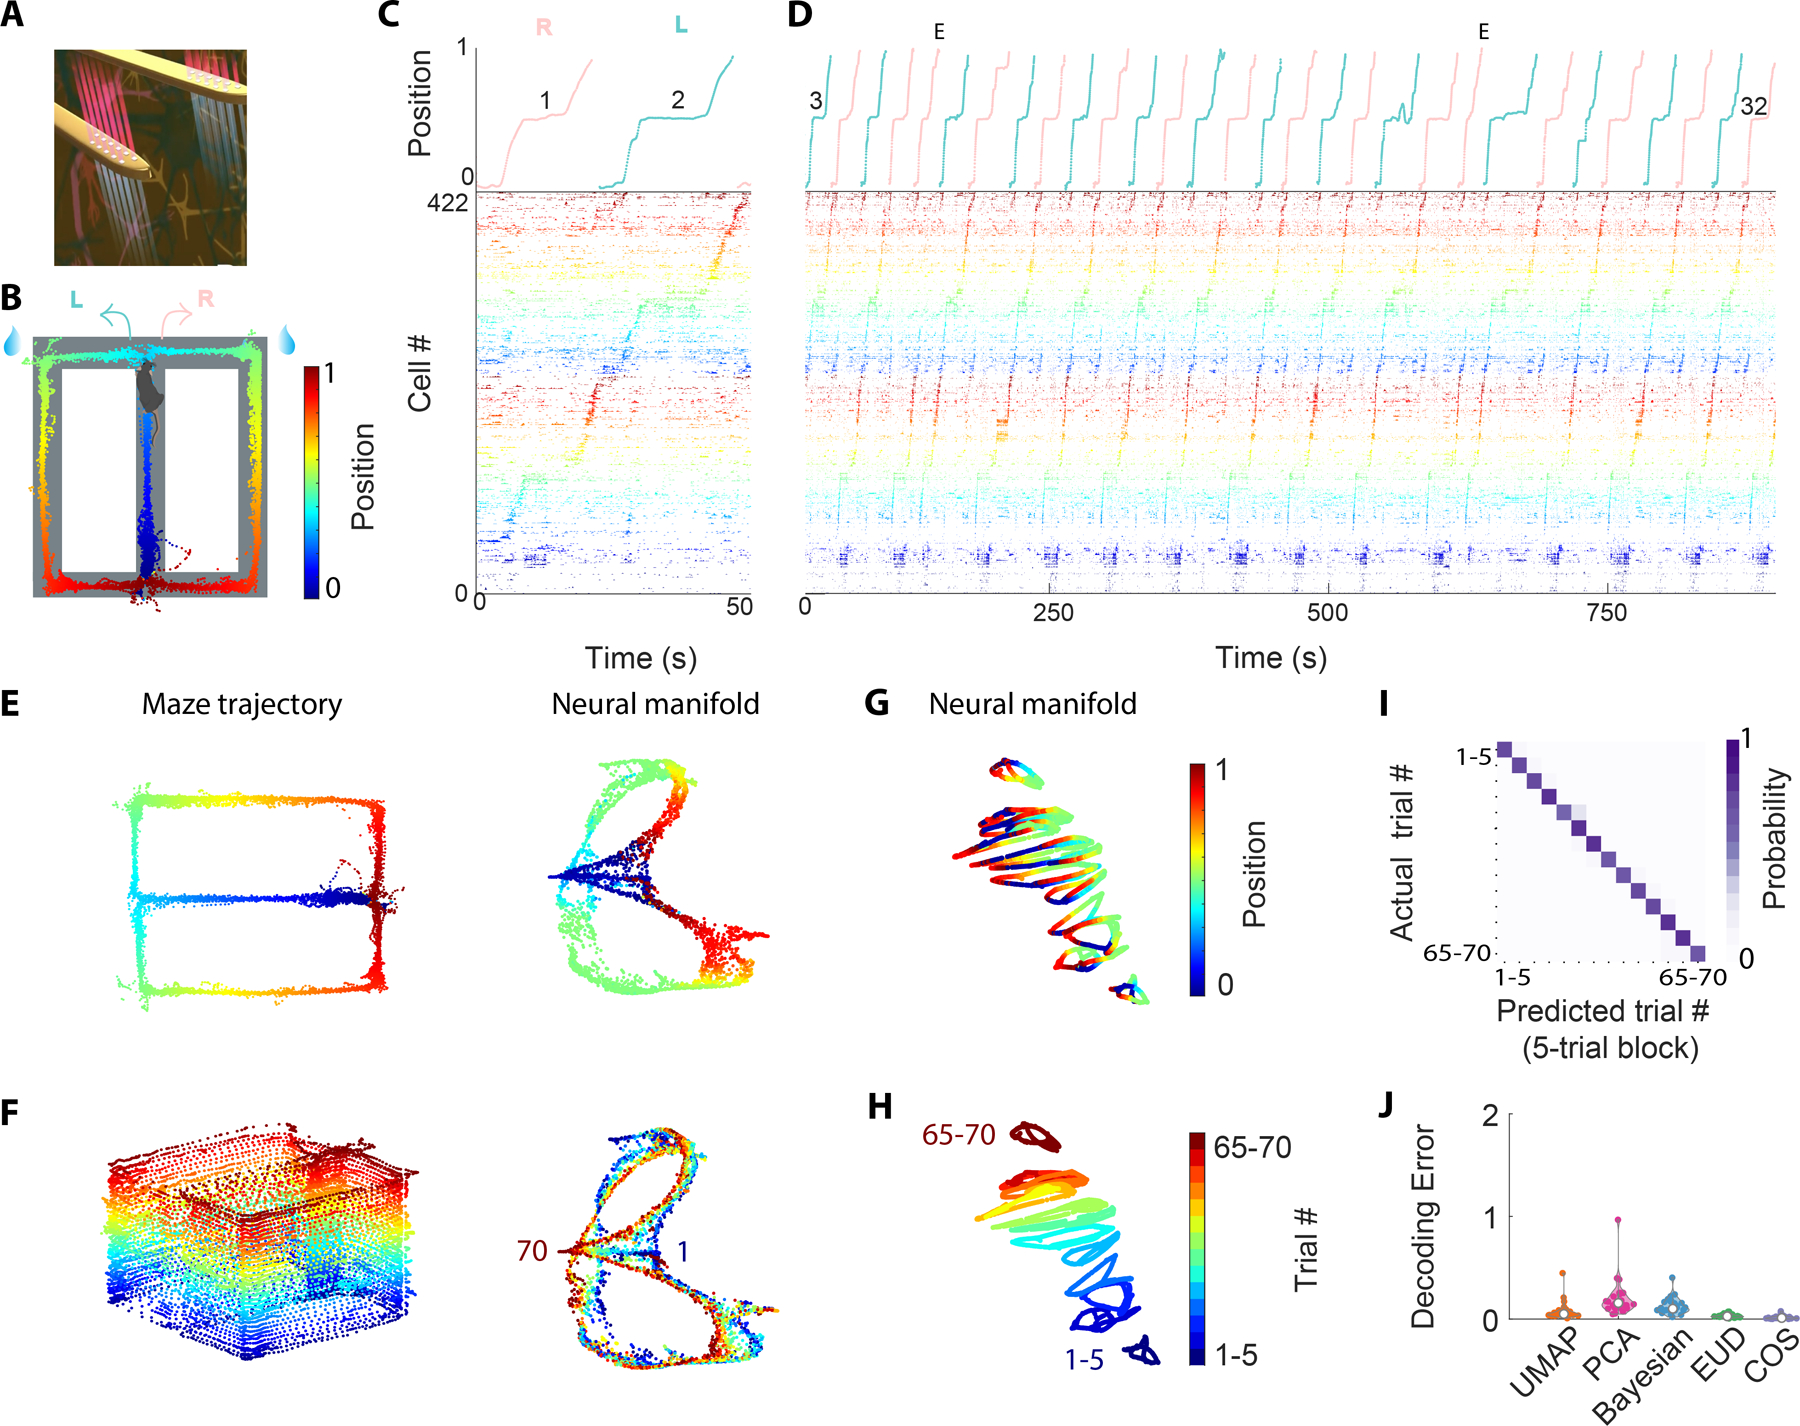
\includegraphics[width=\textwidth]{figures/ch_selection2024/fig1.jpg}
\caption[Trial block identity decoded from neural population activity]{%
\textbf{Trial block identity decoded from neural population activity.}
(A) Illustration of two (out of four) shanks of the dual-sided probe.
(B) The figure-eight maze task, where mice alternated between left and right arms for water reward (blue droplets). The mouse's trajectory along maze corridors is color coded by its linearized position.
(C) Trials 1 (right arm traversal) and 2 (left arm traversal) during the figure-eight maze task. (Top) The linearized position of the mouse. Red, right traversal; green, left traversal. (Bottom) A raster plot of 422 pyramidal cells simultaneously recorded from the right dorsal CA1 region of a mouse's hippocampus, sorted by seqNMF, and color coded according to the linearized position. This follows the same color scheme as in (B).
(D) Trials 3 to 31 (of 70 trials in total) of an example session. E, error trials.
(E) (Left) Running trajectory of a mouse in the figure-eight maze. (Right) UMAP embedding of population activity. Each point corresponds to the low-dimensional embedding of one 100-ms bin of spiking data.
(F) The same session as (E), but the running trajectory and neural manifold are colored by trial block number (see color key in (H)).
(G) Neural manifold of the same session as (E) and (F) made by using semi-supervised UMAP trained on blocks of five trials. The manifold is colored by linearized position.
(H) Same as (G), but the neural manifold is colored by trial block number.
(I) Confusion matrix of trial block decoding from the original high-dimensional space (same session as (A) to (H)).
(J) Trial block identity decoding errors from across all sessions using UMAP, PCA, Bayesian decoding, decoding from original high-dimensional space with Euclidean distance (EUD), and cosine similarity (COS) as distance metrics. Each dot in the violin plot indicates one session, pooled across $n = 26$ sessions from six animals. Decoding error was measured in units of trial block in which five trials were binned to one trial block.
}
\label{fig:selection2024-fig1}
\end{figure}

To quantify the trial sequence information present in the state space, we tested if trial block membership could be accurately decoded from the population activity. Successive five trials composed a trial block, and a specific label was assigned to each trial block. Decoding was performed using a k-nearest neighbor (kNN) decoder, followed by 10-fold cross-validation in the original high-dimensional space. Trial block membership could be accurately decoded from the original high-dimensional space as well as from the low-dimensional UMAP embedding. These results were further confirmed by using principal component analysis (PCA) for dimensionality reduction or by using Bayesian decoding. These findings indicate that inter-trial variation of population activity (drift) cannot be captured by random fluctuations at the single neuron level.

\subsection{Inter-trial variation of population activity is not random}

To probe the contribution of the individual neurons to the aforementioned neuronal population features, we first plotted the tuning curves of individual neurons across trials. We found diverse patterns of inter-trial variability: within-place field rate remapping, place fields emerging on later trials, and shifting place fields across trials. In principle, decodability of trial block membership could be explained by either stochastic or structured variation across trials. To identify the source of variability, we built a model that generated stochastic fluctuation in firing rate across trials. Each simulated cell's spiking activity was generated through a Poisson process based on the tuning curve of real neurons. We passed the simulated spike trains through the same dimensionality-reduction pipeline as we did for the real data. The manifold of the simulated data also reflected the topology of the maze. By contrast, trial block identity information across trials vanished. As an alternative to the standard 10-fold cross-validation method, we implemented a targeted validation method (a ``leave one trial block out'' procedure) that was expected to yield high decoding accuracy only if the state space of the data changed in a structured way, evolving along one axis according to the sequence of trial events.

\begin{figure}[htbp]
\centering
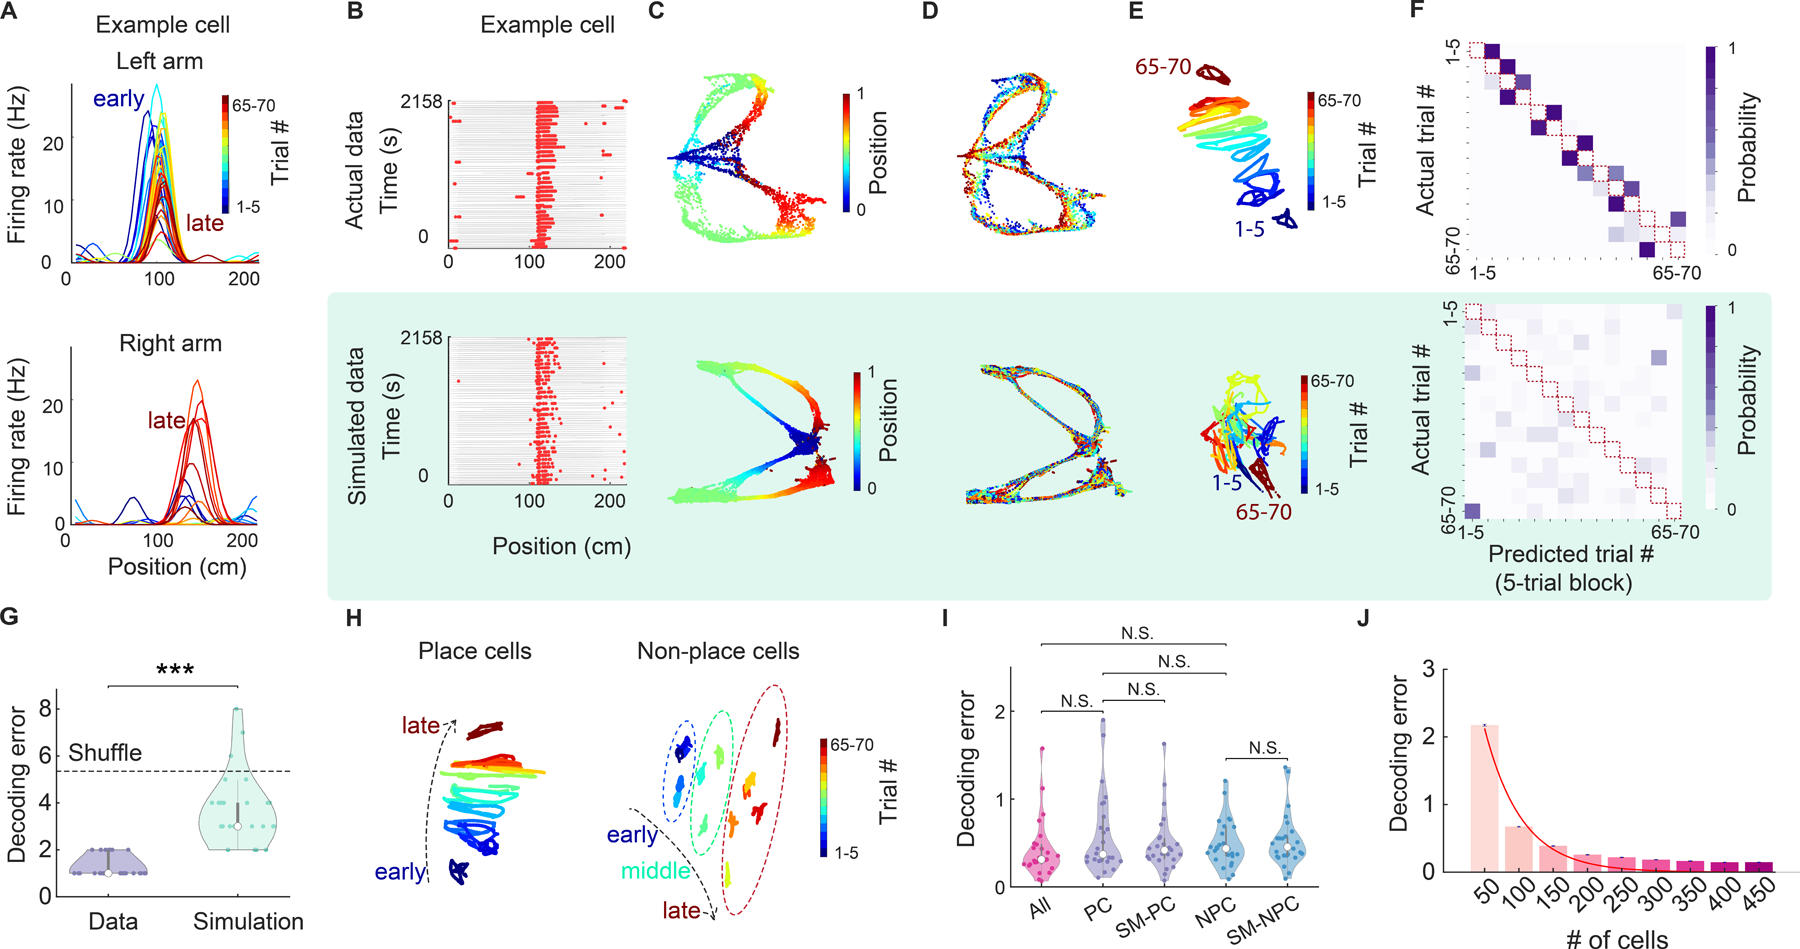
\includegraphics[width=\textwidth]{figures/ch_selection2024/fig2.jpg}
\caption[Contribution of single cell and subpopulation to trial block coding]{%
\textbf{Contribution of single cell and subpopulation to trial block coding.}
(A) Trial-by-trial firing rate of an example neuron during left-arm (top) and right-arm trials (bottom) in the figure-eight maze. Color indicates the trial block number.
(B) Raster plot of an example neuron (top) and a simulated neuron (bottom), generated from a Poisson process model based on the across-trial mean firing rate of the real neuron.
(C) (Top) UMAP manifold generated from the population activity of all the neurons in one example session. (Bottom) UMAP embedding from the simulated population activity. Both are colored by linearized position.
(D) Same as (C) but colored by the trial block number (see color key in (E)).
(E) Neural manifold of the same session as (C) and (D) made by using the semi-supervised UMAP trained on blocks of five trials.
(F) Confusion matrix of trial block decoding results for the real (top) and simulated population (bottom). For decoding results from other decoding methods, see supplementary figures.
(G) Trial block decoding error of real (purple) and simulated (green) data across all sessions (decoded from the original high-dimensional space) (***$P < 10^{-10}$, unpaired t test; $n = 26$ sessions from six animals). The dashed line indicates the chance level from trial-shuffled data.
(H) Neural manifold generated from place cells (left) and nonplace cells (right) from the same session as (A) to (F) by using semi-supervised UMAP trained on blocks of five trials.
(I) Trial block decoding error of all cells (red), place cells (PC), and its size-matched control from all cells (SM-PC, purple), as well as nonplace cells (NPC) and their size-matched control (SM-NPC, blue). Decoding error was measured in units of trial block in which successive five trials were binned to one trial block. (N.S., not significant; unpaired t test; $n = 26$ sessions from six animals.)
(J) Decoding error when downsampling the cells in the example session to subsamples of varying cell numbers (from 50 to 450 cells). Error bar indicates the standard error of the mean (SE) across 1000 subsamples. Decoding error was measured in units of trial block in which successive five trials were binned to one trial block. The red line shows the fitted exponential curve.
}
\label{fig:selection2024-fig2}
\end{figure}

Because the training set did not contain any data that shared the trial block membership with the test set, the test data could decode only to the next closest trial block (not the same trial block) in the state space. Indeed, we observed that only the real data were decoded correctly to the preceding or succeeding trials, occupying the space immediately next to the diagonal of the confusion matrix. The trial decoding accuracy of the real data was significantly higher than that of the simulated or trial-shuffled data. These findings indicate that inter-trial variation of population activity (drift) cannot be explained by electrode drift. Both place cells (PC) and nonplace cells (NPC) contributed to trial block membership decoding. Neural manifolds of different trials were aligned better with place cells than with nonplace cells. Decoding accuracy deteriorated rapidly when downsampled to fewer than 100 neurons in a session, indicating that trial block identity is encoded in the population.

\subsection{Place and trial sequence encoding associated with theta frequency oscillations}

Place and trial sequence encoding is associated with the theta frequency (6 to 9 Hz) oscillations (``theta state'') as animals actively navigate in an environment. When animals stop consuming the water reward, the theta activity gives way to synchronous population events, SPW-Rs. Because spike sequences within SPW-Rs are known to replay place field sequences, we asked whether trial block identity could also be decoded in replay events. A candidate SPW-R event was classified as a significant replay if both its distance to manifold and trajectory length were significantly shorter than those of shuffled distributions. The majority of SPW-Rs occurred in the reward area. About 33\% of the awake SPW-Rs were significant replays.

From the original high-dimensional space, we decoded not only the spatial trajectory but also the trial block identity of the significant replay events. We validated the decoding results using four different methods, including decoding from the original high-dimensional space with different distance metrics and decoding from the low-dimensional space with PCA and UMAP. Different methods yielded consistent decoding results. The within-event coherence of trial replay was high (different time bins within the same events coherently decoded to the same trial block) but decreased rapidly as we downsampled the number of cells included for decoding. Next, we examined whether the SPW-Rs replayed the past, future, or current trial block.

\begin{figure}[htbp]
\centering
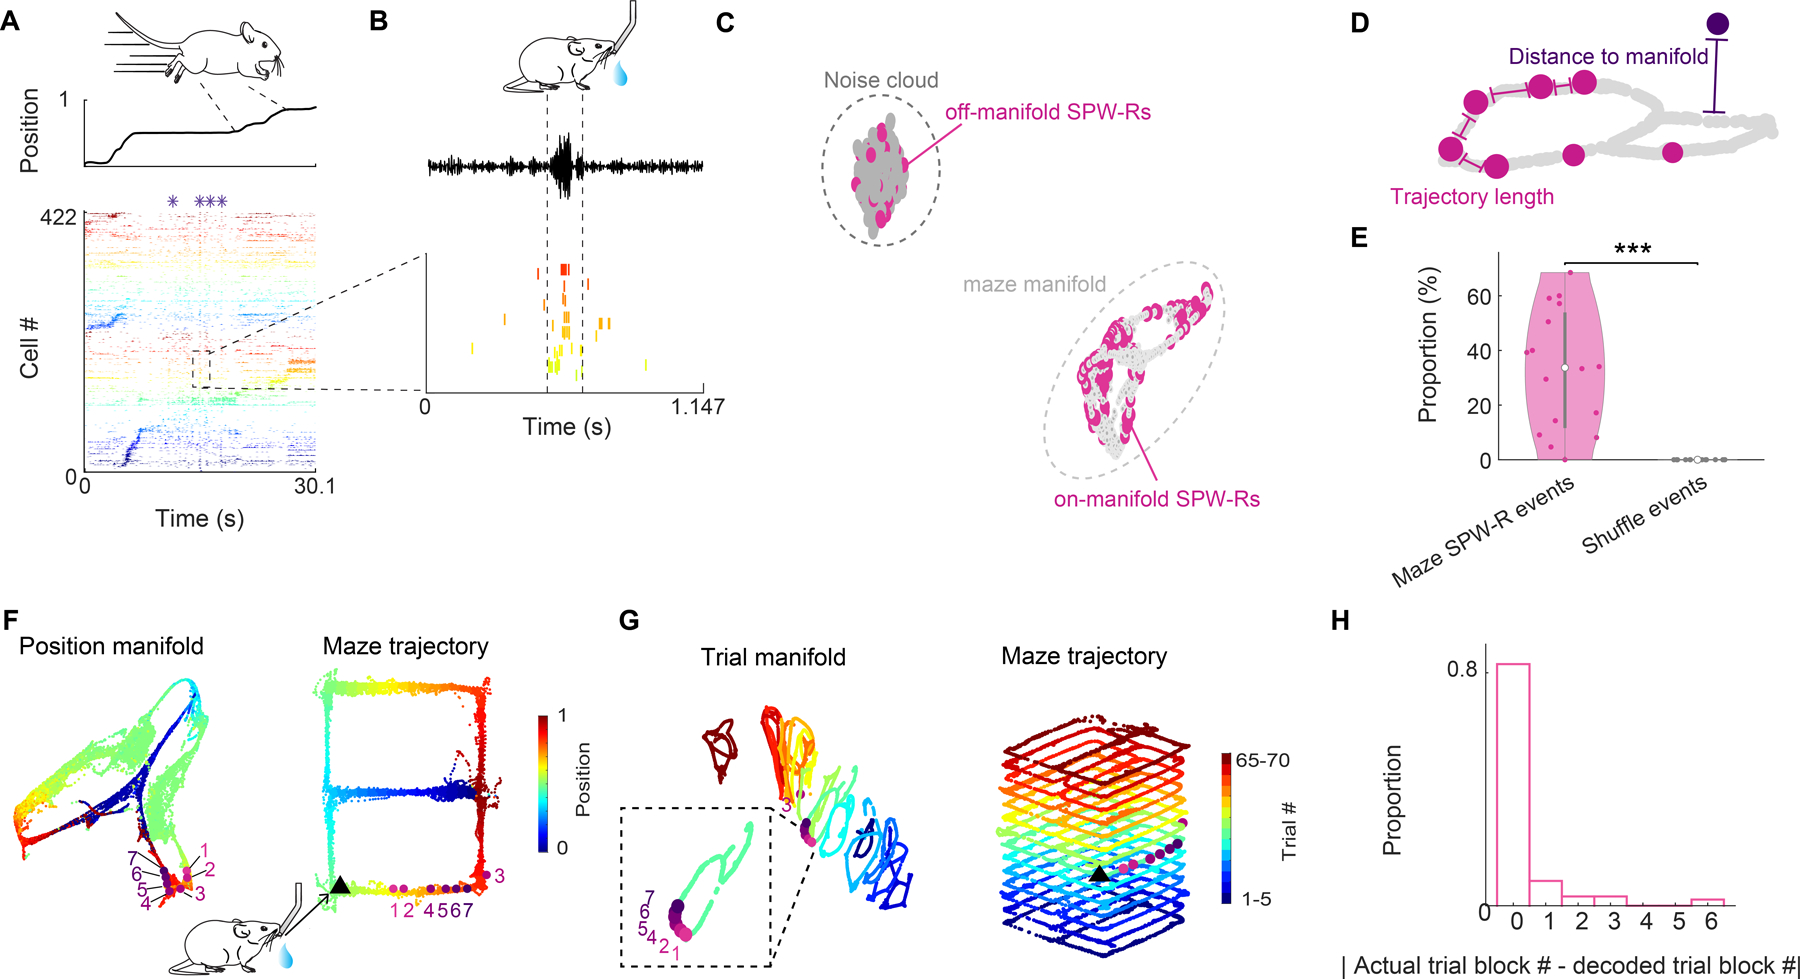
\includegraphics[width=\textwidth]{figures/ch_selection2024/fig3.jpg}
\caption[Maze SPW-Rs replay of trial block identity]{%
\textbf{Maze SPW-Rs replay of trial block identity.}
(A) Spiking activity of an example trial in the figure-eight maze. (Top) Linearized position of the mouse. (Bottom) Raster plot of neuronal spiking activity sorted by seqNMF. Purple stars, SPW-Rs.
(B) Zoomed-in display of a replay event. (Top) Local field potential (LFP) filtered in the ripple band. (Bottom) Raster plot of neurons belonging to a sequence factor with significant reactivation strength. Neurons were sorted in the same order as in (A).
(C) All waking SPW-R events (red) in this example session were embedded with the neural manifold data during navigation (light gray), and the noise cloud consisted of negative samples (dark gray). Two clusters of SPW-R replay events were distinguished: off- and on-manifold events.
(D) SPW-R replays were classified as significant if they were (1) close to the maze manifold and (2) their trajectory length along the manifold was short in comparison to shuffled data.
(E) Percentage of significant replays in the maze (number of significant maze replay events/total number of maze SPW-R events) compared with shuffled data. (***$P < 10^{-4}$, unpaired t test; $n = 26$ sessions from six animals.)
(F) UMAP embedding and the decoded position for the same event as in (B). (Left) The neural manifold during maze running (``position manifold,'' colored by position). (Right) The position content of each replay time bin was decoded to a position bin along the maze trajectory according to the position label of its nearest neighbor on the manifold. The black triangle represents the physical location of the mouse when the replay event took place, and the pink-purple dots represent the neural embedding of seven successive 20-ms time bins of a SPW-R replay event (each time bin was 20 ms).
(G) (Left) The same event was embedded with the ``trial manifold'' and was colored by trial block number. (Right) Trial content of each replay time bin was decoded as the trial block label of its nearest neighbor on the manifold (each trial block corresponds to five trials).
(H) Distribution of differences between the actual trial block of SPW-Rs events and their decoded trial block identity across all sessions.
}
\label{fig:selection2024-fig3}
\end{figure}

The spike content of SPW-Rs decoded most reliably to the present trial block. The strongest predictor of the trial block distribution pattern for maze replay was the immobility time.

\subsection{Post-experience sleep SPW-Rs replay events selected by waking SPW-Rs}

To examine the relationship between awake SPW-Rs and those during post-experience sleep, we compared the population activity of awake SPW-Rs in the maze with that during post-experience sleep in the homecage. The distribution patterns of trial block identity during post-experience sleep were highly correlated with that during maze replay, but not with pre-experience sleep replay. We compared which factor best explained the trial block distribution pattern during post-experience sleep by using a mixed-effect linear regression analysis. All decoding methods consistently showed that the strongest predictor for the trial block distribution pattern during post-experience sleep was that of the SPW-R replay in the maze. We examined whether replays of the left versus right arms during waking and post-sleep SPW-Rs were correlated, exploiting the natural variability in the replay distribution patterns across different arms in different sessions. The correlation of maze-arm replays between wake and sleep SPW-Rs was significantly higher than in the shuffled data. The difference in replay proportion across left and right arms could not be explained by the difference in decodability (measured by spatial information) or the difference in coverage (measured by number of visits) between the two arms.

\begin{figure}[htbp]
\centering
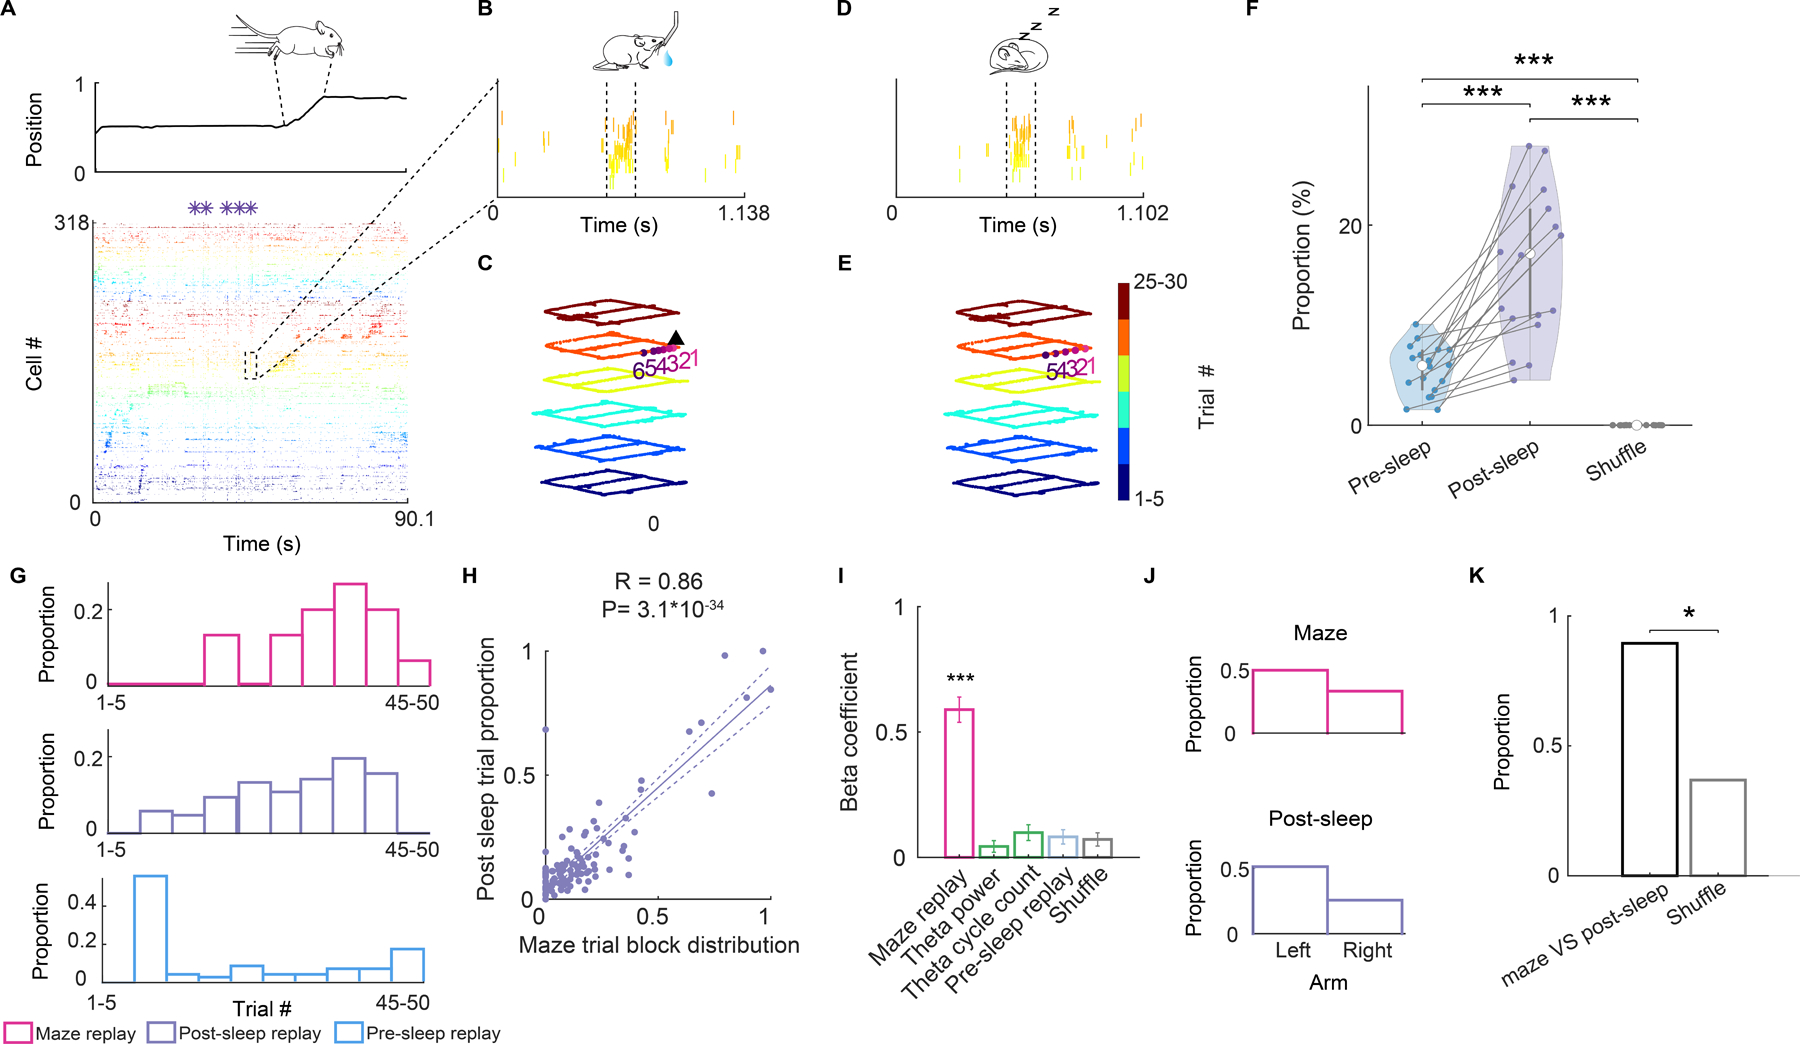
\includegraphics[width=\textwidth]{figures/ch_selection2024/fig4.jpg}
\caption[Replay of trial block identity and maze segments during sleep predicted from waking SPW-Rs]{%
\textbf{Replay of trial block identity and maze segments during sleep predicted from waking SPW-Rs.}
(A) Spiking activity in the figure-eight maze. (Top) Linearized position of the mouse. (Bottom) Raster plot of neuronal spikes, sorted by seqNMF. Purple stars represent SPW-Rs.
(B) Zoomed-in display of an awake replay event in the maze. The raster plot contains neurons belonging to the sequence factor with significant reactivation strength. Neurons were sorted in the same order as in (A).
(C) Decoded position and trial block identity of successive 20-ms bins (one to six bins) of the same SPW-R replay event in (B). The black triangle represents the physical location of the mouse when the replay event took place.
(D) Raster plot of a SPW-R replay event during sleep in the homecage.
(E) Decoded position and trial block identity of successive 20-ms bins of the same SPW-R replay event in panel (D). (A), (B), and (D) were colored according to the linearized position of the mouse; (C) and (E) were colored according to trial block number.
(F) Percentage of significant replays during pre- and post-experience sleep (presleep and postsleep, respectively) in the homecage compared with shuffled data. (Presleep versus postsleep, ***$P < 10^{-5}$; postsleep versus shuffled data, ***$P < 10^{-8}$; presleep versus shuffled data, ***$P < 10^{-8}$; unpaired t test; $n = 26$ sessions from six animals.)
(G) Distribution of the trial blocks decoded from the population spike content of SPW-Rs in an example session. (Top) Maze and postsleep replay trial block distribution pattern. (Bottom) Maze and presleep replay trial block distribution pattern.
(H) Correlation between trial block distributions across trial blocks during maze and postsleep SPW-Rs replay (decoded from the original high-dimensional space; Pearson correlation coefficient, $R = 0.86$; $P < 3.1 \times 10^{-34}$; $n = 16$ sessions from five animals) (results from all four different decoding methods, see supplementary figures).
(I) The predictive relationship between trial block distribution patterns of postsleep SPW-Rs and other candidate variables, including the trial block distribution patterns of the theta cycle, theta power, presleep, and trial-shuffled data (***$P < 10^{-23}$ for awake replay; ***$P < 10^{-3}$ for the theta cycle number; the relative predictive power of a given metric was considered non-significant when it overlapped with zero; $n = 16$ sessions from five animals) (for results from all four different decoding methods, see supplementary figures).
(J) Proportion of maze segment replays (left arm and right arm) during awake and postexperience sleep SPW-Rs in an example session.
(K) Proportion of sessions with same rank order between maze segments during awake and post-maze sleep SPW-R replays, compared with shuffle data. (*$P < 0.05$, chi-square test; $n = 13$ sessions from five animals).
}
\label{fig:selection2024-fig4}
\end{figure}

\section{Discussion}

Waking SPW-Rs weigh and select the experience, and sleep SPW-Rs consolidate it. Exploration of the environment is a regular alternation between ambulation and rest phases, enabling brain state changes. During reward consumption, theta activity gives way to synchronous population events, SPW-Rs. Salient features of the experience, such as novelty, repetition, and reward, increase the incidence of SPW-Rs and replays. In our experiments, we could exclude differences in external factors that could shape sleep replay patterns by demonstrating distinctly changing neuronal population activity patterns within the same maze and session. Selective tagging of trial events by waking SPW-Rs could occur because the perpetually evolving population activity patterns during the theta state serve as a temporal scaffold to organize experiences and differentiate successive events.

The sequence of theta state-dependent turnover of neuronal assemblies, their selection by waking SPW-Rs, and the numerous repetitions during sleep SPW-Rs may represent a hippocampal network mechanism of selective episodic memory consolidation. Our observations suggest that rewards provide an affordance for shifting brain states and that the waking SPW-R serves as a neurophysiological mechanism for memory selection.

These findings establish a neurophysiological framework for multiple domains of systems neuroscience, including credit assignment, representational drift, event remapping, time coding, and memory editing. Our work also links a shared principle of memory processing important for both biological and artificial learning. In particular, it relates to importance sampling in machine learning, which enables faster acquisition and more robust generalization.

Previous observations support this scenario. Cues relevant to future behavioral success can bias the neuronal trajectories of SPW-Rs. Perturbation of SPW-Rs prevents place field and experience stabilization. In humans, items for which electrophysiological brain patterns are not reactivated during non-REM sleep are forgotten. Replay can occur after a single experience and the number of SPW-R after learning predicts subsequent memory performance.

\section{Methods}

\subsection{Implantation and recording}

The data in this paper includes 3 different datasets. Dataset 1 was the main dataset used for both visualization and quantification. Only 1 session was taken from datasets 2 and 3, and shown in Fig. S2 only for visualization. The purpose of the visualization is to demonstrate that the trial block-specific population activity pattern can be observed in diverse tasks and different rodent species.

For Dataset 1, chronic recordings were performed from freely moving adult C57BL/6J mice. The mice were anesthetized with 1.5--2\% isoflurane and implanted with high-density silicon probes, mounted on a microdrive. The ASSY Int64-P32-1D or ASSY Int128-P64-1D silicon probes (Diagnostic Biochips) were dual-sided designs, equipped with recording sites on both sides of each shank. The spacing between shanks was 250-$\mu$m. Craniotomy was drilled at $-2$-mm anteroposterior (AP) and 1.7-mm mediolateral and the probe was lowered to the deep neocortical layers, and the drive was cemented to the skull. A stainless-steel screw was placed over the cerebellum for grounding and reference. Craniotomies were sealed with a mix of dental wax and mineral oil, and a copper mesh cage was constructed to provide electrical and mechanical shielding. Postoperatively, animals received a single intramuscular injection of 0.06-mg/kg of buprenorphine (0.015-mg/ml) as needed for the next 1--3 d. Animals were allowed a 7-d recovery period before the start of experiments. After a 7-d recovery period, neural signals were recorded in the homecage while probes were lowered into the CA1 pyramidal layer, which was identified physiologically via the sharp wave polarity reversal. Neural data were amplified and digitized at 30-kHz using Intan amplifier boards.

For Dataset 2, male Long-Evans rats (250--350 g) were bilaterally implanted in the dorsal hippocampus with two 8-shank (BUZ64) silicon probes. Each shank of the 8-shank silicon probes had 8 sites. All sites were vertically staggered along the shank with 20-$\mu$m spacing between sites. Each site had an area of 160-$\mu$m$^2$ and an impedance of 1--3-M$\Omega$. In each rat, 50-$\mu$m wires were placed gently abutting the left and right mastoid masseter muscle as well as the back neck muscle for electromyographic (EMG) recordings used in sleep classification. All silicon probes were implanted parallel to the septo-temporal axis of the dorsal hippocampus. Finally, each rat was fitted with a small 3-dimensional accelerometer to record the animals' movement, or its absence, during sleep. Two stainless steel screws implanted above the cerebellum were used for referencing and grounding. Each silicon probe was attached to a micromanipulator and lowered over several days until hippocampal layer CA1 was reached as determined by the appearance of hippocampal CA1 sharp wave ripples and pyramidal cell activity.

For Dataset 3, procedures were identical to those for Dataset 1 with the following exceptions: an 8-shank, single sided 128 channel probe (128-8, Diagnostic Biochips) was implanted transversely into the right dorsal hippocampus (medial edge 2.2-mm posterior, 1.1-mm lateral of bregma, lateral edge 1.5-mm posterior and 1.8-mm lateral of bregma). Peri- and postoperative analgesia was performed with subcutaneous Ketoprofen 10 mg/kg daily for 3 days.

\subsection{Behavior}

Mice (Dataset 1) were trained on a spatial alternation task in a figure-eight maze and linear maze. Animals were water-restricted before the start of experiments and familiarized with the maze raised 61 cm above the ground. Several days after the start of water deprivation, animals were shaped to visit alternate arms between trials to receive a water reward in the first corner reached after making a correct left/right turn. A 5-s delay in the start area was introduced between trials. Infrared (IR) sensors were used to detect the animal's progression through the task and 3D-printed doors mounted to servo motors were opened/closed to prevent the mice from backtracking. The position of head-mounted red LEDs was tracked with an overhead Basler camera at a frame rate of 30 Hz, and tracking data were aligned to the recording via TTL pulses from the camera, as well as a slow pulsing LED located outside the maze. In all sessions that included behavior, animals spent approximately 120 min in the homecage before running on the maze and another approximately 120 min in the homecage afterward. All behavioral sessions were performed in the mornings (the start of the dark cycle). Only sessions with more than 150 cells and more than 20 trials were selected for analysis. $n = 26$ sessions from 6 animals (21 out of 26 sessions were figure-8 maze sessions, and 5 of them were linear maze sessions).

For Dataset 2, a rat (Achilles) was extensively handled both before and after surgery. Water restriction was initiated one week after the surgery; animals were restricted to 90\% of their initial body weight and given one day a week of ad lib water access. The rat was well acclimated and recorded in the ``familiar'' room (where all sleep recordings were performed) for at least one week prior to novelty maze sessions.

For Dataset 3, the mouse was handled and familiarized with the maze for multiple days prior to the commencement of experiments. It was then trained to forage for rewards on the radial 8-arm maze. The maze consisted of eight concentrically arranged arms of hard plastic (each arm 40-cm long) with 50-cm high side walls that were elevated 30-cm above the floor. In this version of the task, three out of the eight arms of the maze were chosen semi-randomly every day, with the constraints that a maximum of two adjacent arms were rewarded and that at least 2 arms had to be different from those of the previous day. These three arms were initially ``baited'' with water rewards but only re-plenished after the animal had visited all rewarded arms. There were no discrete trials and the animals were allowed to continuously forage the maze for 20 minutes. The animal was then placed in its home cage for 2 hours, during which neuronal activity was recorded.

\subsection{Unit isolation and classification}

Spikes were extracted and classified into putative single units using KiloSort1 and manual curation was performed in the Phy2 software with the aid of customized plugins.

\subsection{Place field and spatial information}

Place field analysis was done using standard methods. The firing rate distribution within place fields (``rate map'') was generated by first binning spiking data into 5-cm wide bins, and spike counts were normalized by time occupancy (smoothing size: 2-bins). Trials for forward and backward directions were evaluated separately. The field boundaries were defined when the rate decreased below 20\% of the peak firing rate. Place fields cleared all criteria when they were between 8.75-cm and 75-cm wide, had a minimum peak firing rate of 3-Hz, and had a spatial coherency $> 0.7$.

Spatial information was calculated in bits per spike as:
\[
\text{SPI} = \sum_i p_i \log_2 \left( \frac{\lambda_i}{\lambda} \right)
\]
where $\lambda_i$ is the mean firing rate of a unit in the $i$-th bin, $\lambda$ is the overall mean firing rate and $p_i$ is the probability of the animal being in the $i$-th bin (occupancy in the $i$-th bin / total recording time).

\subsection{Poisson process for modeling single cell activity across trials}

The simulated spike was modeled based on a Poisson process:
\[
\Pr(X = \kappa) = \frac{\lambda^\kappa e^{-\lambda}}{\kappa!}
\]
The procedure to generate Poisson spikes followed previous work. For each simulated neuron, the spike train progresses through time in small windows of $dt$ (1-ms), and spikes were generated via Poisson process using the cross-trial mean firing rate $fr(pos)$ of the real neuron at position $pos$.

\subsection{Theta-cycle detection}

Theta cycle detection was done following standard procedures. Broadband LFP was bandpass filtered between 6 and 12-Hz using a fourth-order Chebyshev filter. The Hilbert transform of the filtered signal was computed, and its absolute value and angle at each timepoint were taken to be the theta-band amplitude and phase, respectively. Intervals with theta-band amplitude 1 s.d. above the mean were considered for theta cycle detection. Within these intervals, timepoints where the phase crossed 0$^\circ$, were identified as peaks of theta, and timepoints of consecutive theta peaks were considered the onsets and offsets of individual theta cycles. Only theta cycles occurring within identified awake periods were considered for analysis.

\subsection{State scoring}

State scoring was performed as described previously. The LFP was extracted from wideband data by low-pass filtering (sinc filter with a 450-Hz cut-off band) and downsampling to 1,250-Hz. Three signals were used for state scoring: broadband LFP, narrowband theta frequency LFP and electromyogram (EMG). Spectrograms were computed from broadband LFP with fast-Fourier transform in 10-s sliding windows (at 1-s) and principal component analysis (PCA) was computed after a z transform. The first PC reflected power in the low ($< 20$-Hz) frequency range, with oppositely weighted power at higher ($> 32$-Hz) frequencies. Theta dominance was quantified as the ratio of powers in the 5 to 10-Hz and 2 to 16-Hz frequency bands. EMG was estimated as the zero-lag correlation between 300 and 600-Hz filtered signals across recording sites. Soft sticky thresholds on these metrics were used to identify states. High LFP PC1 and low EMG were taken to be NREM, high theta and low EMG were considered to be REM and the remaining data were taken to reflect the awake state. All assignments were inspected visually and manually curated wherever appropriate.

\subsection{Ripple detection}

Ripple events were conditioned on the coincidence of both population synchrony events and LFP detected ripples. For each session the combined spiking of all recorded CA1 pyramidal cells was binned in 1-ms bins and convolved with a 15-ms Gaussian kernel. For each session, a trigger rate was defined as being 3 standard deviations above the mean of all 1-ms bins within NREM epochs of both PRE and POST epochs combined. Putative population synchrony events were detected when the smoothed firing rate vector crossed the trigger rate. The beginning and end of the putative synchrony events were defined as the time points at which the convolved firing rate vector returned to the mean of all within-NREM firing rate bins. Independently, ripple events were detected from the pyramidal layer LFP. Population synchrony events that did not contain at least one LFP-detected ripple were discarded. Population synchrony events that (1) contained at least one LFP-detected sharp wave-ripple, (2) lasted between 50 to 500-ms, (3) occurred during non-theta or ``off-line'' states (quite awake immobility or NREM) and (4) in which at least five distinct pyramidal cells each fired at least one spike were termed ``Ripple events'' and considered for further analysis. This ``five pyramidal cells'' inclusion criterion was used as it is the minimum number of cells needed to establish significance for sequence relationship between cells at $p < 0.05$.

\subsection{SeqNMF}

SeqNMF algorithm was implemented using existing methods and code. Briefly, seqNMF started by taking a data matrix $X$ which contains the activity of $N$ neurons at $T$ time points. If the neurons exhibit a single repeated pattern of synchronous activity, the entire data matrix can be reconstructed using a column vector $w$ representing the neural pattern and a row vector $h$ representing the times and amplitudes at which the pattern occurs. Data matrix $X$ was mathematically reconstructed as the outer product of $w$ and $h$. If multiple component patterns are present in the data, then each pattern can be reconstructed by a separate outer product, where the reconstructions are summed to approximate the entire data matrix as follows:
\[
X \approx \sum_{k=1}^K W_{nk} H_{kt} = (WH)_{nt}
\]
where $X_{nt}$ is the ($nt$)-th element of matrix $\mathbf{X}$, which represents the activity of neuron $n$ at time $t$. To store $K$ different patterns, $\mathbf{W}$ is an $N$ by $K$ matrix containing the $K$ exemplar patterns or sequence factors and $\mathbf{H}$ is a $K$ by $T$ matrix. For these experiments, $K = 8$ was chosen, given the topology of the figure 8 maze.

\subsection{Assessment of single unit stability across trials}

The displacement of the estimated positions of single units relative to the probe sites was measured following previous descriptions. The centroid of each single unit was measured by a spatial average across electrode positions weighted by the square of the mean waveform amplitude at each electrode.

\subsection{Low-dimensional manifold visualization with UMAP (unsupervised)}

Neural data were first preprocessed before dimensionality reduction. Neural spiking data (spike count) during maze learning was binned into 100-ms bins. The data was then smoothed using a 500-ms wide Gaussian kernel and z-scored. The UMAP dimensionality reduction algorithm was then applied to this matrix. Each point in the low-dimensional manifold corresponds to the population activity at a single time bin in the session. UMAP hyperparameters used were: $n\_neighbors = 20$, $metric =$ `cosine', $output\_metric =$ `euclidean', $learning\_rate = 1.0$, $init =$ `spectral', $min\_dist = 0.1$, $spread = 1.0$, $repulsion\_strength = 1.0$, $negative\_sample\_rate = 5$, $target\_metric =$ `categorical', $dens\_lambda = 2.0$, $dens\_frac = 0.3$, $dens\_var\_shift = 0.1$.

\subsection{Low-dimensional manifold visualization with UMAP (supervised)}

With supervised methods, data from the same trial were given the same label. Data points that share the same labels were leveraged so that similar points were embedded closer together. This was implemented by passing the trial block number as target when calling the fit-transform function from the UMAP python package.

\subsection{Decoding maze data with UMAP}

The UMAP dimensionality reduction process was comprised of the following two main steps. First, a weighted k nearest neighbor (kNN) graph, which connects each datapoint to its $k$ nearest neighbors, was constructed and used to generate the initial topological representation of the data from the high-dimensional space. Second, UMAP optimizes the low-dimensional representation to have as close a topological representation as possible to that in the original high-dimensional space.

To decode the trial block identity from population activity, metric learning was implemented. A subset of data was selected as training data, based on which the manifold embedding was generated. The training data was supervised with trial block labels by concatenating 5 trials as one block. After generating the manifold with training data, previously unseen (and unlabeled) test points were then embedded into the learned space using the transform function. The scikit-learn implementation of k-Nearest Neighbors (kNN) algorithm was used to decode the trial block identity of the test data embedded in the low-dimensional manifold. The mode of the three nearest neighbors' trial block membership was taken as the decoded trial block. Position bin membership was decoded following an analogous procedure, using the mode of the three nearest neighbors' position bin membership (5-cm bin).

\subsection{Decoding error and cross-validation method}

Decoding error during behavior was cross-validated by tenfold cross-validation, which was implemented by splitting the data into 10 subsamples, each randomly drawn from across the entire session. Decoders were then trained on 9 of the subsamples and tested on the remaining subsample. All 10 subsamples were used as test data during successive iterations. Decoding error was taken as the average error across all 10 trained decoders. For PCA decoding, cross-validation was repeated 1,000 times with overall decoding accuracy taken as the mean across the 1,000 repetitions.

To test whether the state space of different trials evolved systematically along a single axis (whereby neighboring trial blocks were embedded closer together in the neural manifold), a targeted validation method was also implemented. In contrast to tenfold cross-validation, an entire trial block was held out for each subset of training data. Since the training data did not contain any data that shared the same trial block label with the test data, test data was expected to be decoded to the neighboring trial block only if the population activity of neighboring trial blocks was more similar than that of distant trials. Statistical significance for decoding error was determined by comparing the mean decoding error from the original data against the mean decoding error from trial-shuffled data.

For comparing decoding accuracies across different subpopulations of place cells and non-place cells, size-matched populations were used as control. For the downsampling analysis, different subsets of cells were randomly drawn from the total population of cells for a given session without replacement. For each sample size, 1000 different random seeds were used to randomly subsample different cells. Decoding accuracy was taken as the average accuracy across all 1000 different random samples.

\subsection{Decoding from the original high-dimensional space}

For decoding from the high-dimensional space, the mode of the k nearest neighbors' trial block membership was computed. Two types of distance metrics, Euclidean and Cosine similarity, were used to build the k-neighbor graph. The main summary statistics in the main figures were performed in the original dimensional space.

\subsection{Decoding SPW-R content with UMAP}

Spike trains during maze running were binned into 100-ms time bins, smoothed, and z-scored. Spike trains of candidate SPW-R replays were binned in 20-ms time bins, smoothed, and z-scored. The preprocessed data matrix was then passed through the nonlinear dimensionality reduction step by UMAP, which generated a six-dimensional embedding. Candidate ripple events were embedded with the manifold generated from maze data. For each event, distance to manifold and trajectory length were measured. A candidate event was classified as significant if (1) the mean distance to manifold of a candidate event is significantly smaller than shuffled data (circular shuffle) and (2) the mean trajectory length is significantly smaller than shuffled data (temporal shuffle). For significant replay events, position bin and trial block membership were decoded by embedding the ripple activity vectors with the position manifold and trial manifold, respectively. Each point on the manifold was associated with position bin labels (positions were binned into 5-cm bins) or trial block labels (trials were binned into 5-trial bins). The low-dimensional embeddings along with position or trial block labels were used to train a kNN decoder.

\subsection{UMAP decoding and negative sampling}

At the implementation level, UMAP used a sampling-based approach called negative sampling to optimize the low-dimensional embedding. Data far away from the original high-dimensional space were sampled as negative samples from which data points are repulsed away, whereas similar data in the high-dimensional space were attracted to each other. Negative samples were generated from shuffled data (shuffling the rows and columns of the maze firing rate matrix). With the presence of the negative samples, population vectors similar to the maze manifold were attracted to the maze manifold in the low-dimensional space and those dissimilar to the maze manifold were pulled closer to the negative sample cloud.

\subsection{Criteria for significant replay}

Candidate events were binned into 20-ms bins. Two kinds of shuffles were used to generate a null distribution for distance-to-manifold and trajectory length, respectively: (1) Circular shuffle, which degrades the coordinated population pattern without affecting trajectory length and other properties such as firing rate and firing rate variance of each neuron, and (2) Temporal shuffle, which specifically disrupts the sequence structure of the event while preserving the distance-to-manifold. A replay event was classified as a significant event only when its distance to the manifold was significantly shorter than the circular shuffle and its trajectory length was significantly shorter than the temporal shuffle.

\subsection{Decoding with a Bayesian decoder}

For Bayesian decoding, neural spiking data was preprocessed similarly to UMAP decoding. The data was then smoothed using a 1000-ms wide Gaussian kernel. Only data with speed larger than 2--5-cm/s was used to build the template. Bayesian decoding was performed independently for the left and right arm trials. For each ripple event, the position and trial block identity of the event were decoded separately. For position decoding, Bayesian classification of virtual position was performed utilizing a ``template'' comprising all place cell's firing rate-by-position vector. For trial decoding, Bayesian classification of trials utilized a template comprising all cell's smoothed firing rate-by-position-trial matrix from each arm.

\subsection{Mixed-effect linear regression analysis}

To quantify the relative magnitude of the effects of different variables to explain the trial block distribution pattern of post-sleep replay, mixed-effect linear regression analysis was applied. The model was fitted with the formula:
\begin{align*}
\text{post sleep trial replay pattern} &\sim \text{maze replay trial pattern} \\
&+ \text{theta cycle trial pattern} \\
&+ \text{theta power trial pattern} \\
&+ \text{pre sleep trial pattern} \\
&+ \text{shuffle trial pattern} + \text{(session)}
\end{align*}

\subsection{Statistical analyses}

All statistical analyses were performed with custom-written scripts in MATLAB and Python. Power analysis was not used to determine sample sizes.
